\documentclass[letterpaper, 10 pt, journal, twoside]{IEEEtran}  % Use this command for final RAL version
%\documentclass[a4paper, 10pt, conference]{ieeeconf}      % Use this line for a4 paper

\IEEEoverridecommandlockouts                              % This command is only needed if
                                                          % you want to use the \thanks command

%\overrideIEEEmargins % Needed to meet printer requirements.

\usepackage{mathtools} 
\usepackage{graphicx,subcaption} % to use subfigure
\graphicspath{{img/}}
% To import svg, and automatic workflow with inkscape.
% But including svg also includes subfig which seems to collide with subfigure
% This gives the error main.tex|143 error| Undefined control sequence. \sf@counterlist
% Just remove deprecated subfigure, and use subcaptions instead...
%\usepackage[svgpath=img/]{svg}
% To import pgf figures.
\usepackage{pgf}
% To use svgscale before calling input on a pdf_tex file or svg
\usepackage{calc}
% To solve the issue of relative paths inside pgf.
\newcommand\inputpgf[2]{{
\let\pgfimageWithoutPath\pgfimage
\renewcommand{\pgfimage}[2][]{\pgfimageWithoutPath[##1]{#1/##2}}
\input{#1/#2}
}}

\usepackage{todonotes}
%\global\long\def\todoblue#1{\todo[inline,backgroundcolor=cyan]{#1}}
%\global\long\def\todogreen#1{\todo[inline,backgroundcolor=green]{#1}}
\usepackage{soul}

% To solve a bug with titlesec, and with makeidx
\usepackage{etoolbox}

\usepackage{amsmath} % To get math functionality
% Use amsmath to create my own definition equality symbol
\newcommand\defeq{\mathrel{\overset{\makebox[0pt]{\mbox{\tiny def}}}{=}}}
\usepackage{amssymb} % For nice math symbols
\usepackage{bm} % Better than \boldsymbol, use \bm
\usepackage[export]{adjustbox}% http://ctan.org/pkg/adjustbox
% To add tables with even width
\usepackage{tabularx}
\newcolumntype{Y}{>{\centering\arraybackslash}X} % To make columns content centered
\usepackage{tikz} % To draw
\usetikzlibrary{bayesnet} % To draw factor graphs in latex.

% Set variables for factor graph distances.
\newlength{\state} % Edge distance btw states
\setlength{\state}{1cm}

% For URLs
\usepackage{url}
% For mulicolumn
\usepackage{array}
% For copyright letters
\usepackage{textcomp}
% To avoid commands ignoring space after
\usepackage{xspace}
% To do nice minimalistic tables
% and better spacing above and below the various rules in the table
\usepackage{booktabs}
% To have footnotes in tables
\usepackage{tablefootnote}
% To allow for letters in enumerate (i, ii, ...)
\usepackage[shortlabels]{enumitem}

% For links
\usepackage{hyperref}
% Nice links and urls
\hypersetup{
    colorlinks,
    linkcolor={red!50!black},
    citecolor={blue!50!black},
    urlcolor={blue!80!black}
}

% Cleverer referencing
% Hyperref must be set before cleveref or cref won't work
\usepackage{cleveref}
%\crefformat{section}{\S#2#1#3} % Change section word for symbol
%\crefformat{subsection}{\S#2#1#3}
%\crefformat{subsubsection}{\S#2#1#3}

% Increase secnumdepth to also be able to reference paragraphs
\setcounter{secnumdepth}{6}

% For citations to be ordered
\usepackage[sort]{cite} % sorting is default actually

% useful comments
\usepackage{color}
\newcommand{\Rebuttal}[1]{\textcolor{black}{#1}}
\definecolor{orange}{RGB}{255,127,0}
\newcommand{\TR}[1]{\textcolor{orange}{{\\ \bf TR:}~#1}\\}
\newcommand{\LC}[1]{\textcolor{red}{{\bf LC:}~#1}}

% COLORS
\newcommand{\blue}[1]{{\color{blue}#1}}
\newcommand{\green}[1]{{\color{green}#1}}
\newcommand{\red}[1]{{\color{red}#1}}

% TO MANAGE REFERENCES
%============================================================================
\newcommand{\linkToPdf}[1]{\href{#1}{\blue{(pdf)}}}
\newcommand{\linkToPpt}[1]{\href{#1}{\blue{(ppt)}}}
\newcommand{\linkToCode}[1]{\href{#1}{\blue{(code)}}}
\newcommand{\linkToWeb}[1]{\href{#1}{\blue{(web)}}}
\newcommand{\linkToVideo}[1]{\href{#1}{\blue{(video)}}}
\newcommand{\award}[1]{\xspace} % {{\red{#1}}} % omit awards

\newcommand{\mysubsection}[1]{{\bf#1.}} % \subsection{}

%\title{
%Densifying Sparse VIO \\ A mesh-based approach using structural regularities
%}
\title{Semantic 3D Mesh VIO}

% Paper headers
\markboth{IEEE Intelligent Robots and Systems. Preprint Version.}
{Rosinol \MakeLowercase{\textit{et al.}}: Semantic 3D Mesh VIO}
% Use only for final RAL version

\author{Antoni Rosinol$^{1}$, Siyi Hu$^{1}$, Luca Carlone$^{1}$
\thanks{$^{1}$A.\,Rosinol, S.\,Hu and L.\,Carlone are with the Laboratory for
Information \& Decision Systems (LIDS), Massachusetts Institute of Technology, Cambridge, MA, USA,
{\sf \{arosinol,siyihu,lcarlone\}@mit.edu}}
\thanks{This work was partially funded by ARL DCIST CRA W911NF-17-2-0181.}}%

%\thanks{Manuscript received: September, 10, 2017; Revised December, 2, 2017; Accepted December, 4, 2017.} %Use only for final RAL version
%Use only for final RAL version.

\newcommand{\TODO}[1]{
\textcolor{orange}{{\textbf{TODO:}}~#1} % Comment this line to remove TODOs
}

\input{./chapters/shortcuts} % Shortcuts used by Forster15icra.

\begin{document}

\LC{add: ``Probabilistic Structure from Motion with Objects (PSfMO)''}
\LC{add: ``ObjectFusion: An Object Detection and Segmentation framework with RGB-D SLAM and Convolutional Neural Networks
G Tian, L Liu, JH Ri, Y Liu, Y Sun - Neurocomputing, 2019''}
\LC{add: [PDF] GEN-SLAM: Generative Modeling for Monocular Simultaneous Localization and Mapping
P Chakravarty, P Narayanan, T Roussel - arXiv preprint arXiv:1902.02086, 2019}

\LC{add: [PDF] GEOMetrics: Exploiting Geometric Structure for Graph-Encoded Objects
EJ Smith, S Fujimoto, A Romero, D Meger - arXiv preprint arXiv:1901.11461, 2019}

\LC{Mesh Based Semantic Modelling for Indoor and Outdoor Scenes
Julien P. C. Valentin1,3 Sunando Sengupta1,3 Jonathan Warrell1 Ali Shahrokni2 Philip H. S. Torr1}

\LC{work from Soatto}

\LC{https://journals.sagepub.com/doi/abs/10.1177/0278364919839761}

\maketitle
%\thispagestyle{empty}
%\pagestyle{empty}

%!TEX root = ../main.tex
\begin{abstract}
    We present a suite of algorithms and simulators with open-source implementations suitable for general Robotics development.
    As robotics is starting to have an increasingly important role with applications such as drone delivery and autonomous cars, it is ever more important to test, refine and provide a proof-of-concept of our algorithmic designs in a fast yet reliable way.
    With the advent of powerful desktop computers with multiple graphic cards and high-performance processors, we have the possibility to accurately simulate worlds that are always closer to being indistinguishable from the real world.
    Although we still have not reach the level where one might discard completely a real-life demonstration for the sake of proving the validity of a system, we are getting there at an exponential pace.
    Soon we might reach the point where we will have difficulties to decide what is real from what is computer-generated. If the reader is not convinced that this will happen, we suggest checking the latest developments in Generative Adversarial Networks \TODO{cite}.

    Classical implementations of Visual-Inertial Odometry (VIO) algorithms ignore semantic information of the scene, as they rely solely on sparse landmarks.
    Nevertheless, recent work has shown the advantage of using richer representations of the scene, such as 3D meshes, to extract higher-level information such as structural regularities.
    In this work, we show that a 3D mesh of the scene can be further utilized to accommodate semantic information, which enhances the mapping side of a classical VIO beyond a sparse and uninformative point-cloud.
    Towards this end, we use recent work on semidefinite programming and conditional random fields to generate semantic information in real-time on a single-core CPU.
\end{abstract}

% Keywords appear just beneath the abstract. Use only for final version.
\begin{IEEEkeywords}
Vision-Based Navigation, Semantic Segmentation.
\end{IEEEkeywords}

\vspace{-2em}
\section*{Supplementary Material}
Videos of the experiments: \TODO{Add video url}



%!TEX root = ../main.tex

\section{Introduction}
\label{sec:introduction}

% Drop letter for first word of the Introduction
% Use only for final version.
 \IEEEPARstart{T}{he} advent of drone racing competitions such as \TODO{cite alpha pilot} requires the estimation of the fastest possible trajectory through a given race track.
 Finding this optimal trajectory can be useful for human pilots, and their tacticians, to evaluate their performance and improve upon it.
 For example, the teams in the Red Bull Air Race \TODO{cite redbull and SH} make extensive use of such information to train and perfect their manouevers.
 In this same way, drones can autonomously follow a dynamically feasible trajectory with high accuracy.
 Therefore being able to infer the optimal feasible trajectory could potentially make fully-autonomous drones beat human pilots.
 We are still not there, but great progress in this direction is being made.

{\bf Contributions.}
\begin{itemize}
  \item Formulation of the minimum-time problem for the specific problem of drone-racing through multiple gates.
  \item Presentation of a means to solve the problem using readily available software.
\end{itemize}

{\bf Paper Structure.}
Section~\ref{sec:mathematical_formulation} presents the mathematical formulation of our approach, and discusses the implementation of
Section~\ref{sec:results} reports and discusses the experimental results and comparison against related work. Section~\ref{sec:conclusions} concludes the paper.

%!TEX root = ../main.tex

\section{Related Work}
\label{sec:related_work}

\subsection{}
\label{ssec:sota_vin}

\subsection{Optimal Control}
\label{ssec:sota_optimal_control}
%!TEX root = ../main.tex

\section{Approach}
\label{sec:mathematical_formulation}

\TODO{Apprach}
We consider a stereo visual-inertial system and adopt a \emph{keyframe}-based approach~\cite{Leutenegger15ijrr}.
This section describes our VIO front-end and back-end.
Our front-end proceeds by building a 2D Delaunay triangulation over the 2D keypoints at each keyframe.
Then, the VIO back-end estimates the 3D position of each 2D keypoint, which we use to project the 2D triangulation into a 3D mesh.
While we incrementally build the 3D mesh, we restrict the mesh to the time-horizon of the VIO optimization, which we formulate in a fixed-lag smoothing framework~\cite{Qin17arxiv, Carlone17icra-vioAttention}.
The 3D mesh is further used to extract structural regularities in the scene that are then encoded as constraints in the optimization problem.

%%%%%%%%%%%%%%%%%%%%%%%%%%%%%%%%%%%%%%%%%%%%%%%%%%%%%%%%%%%%%%%%%%%%%%%%%%%%%%%%%%%%
\subsection{Front-end}
\label{ssec:frontend}

Our front-end has the same components as a keyframe-based indirect visual-inertial odometry pipeline\cite{Leutenegger15ijrr, Blosch15iros}, but it also incorporates a module to generate a 3D mesh, and a module to detect structural regularities from the 3D mesh.
We refer the reader to \cite[Sec. 4.2.1]{RosinolMT} for details on the standard modules used, and we focus here instead on the 3D mesh generation and regularity detection.

\subsubsection{3D Mesh Generation}
\label{sssec:3d_mesh_generation}

Building a consistent 3D Mesh of the environment using a sparse point cloud from VIO is difficult because (i) the 3D positions of the landmarks are noisy, and some are outliers; (ii) the density of the point cloud is highly irregular; (iii) the point cloud is constantly morphing: points are being removed (marginalized) and added, while the landmarks' positions are being updated at each optimization step.
Therefore, we avoid performing a 3D tetrahedralisation directly from the sparse 3D landmarks, which would require expensive algorithms, such as space carving \cite{Pan2009proforma}.

\subsubsection{3D Mesh Propagation}
While some algorithms update the mesh for a single frame \cite{Greene17iccv,Teixeira16iros}, we attempt to maintain a mesh over the receding horizon of the fixed-lag smoothing optimization problem (\cref{ssec:backend}), which contains multiple frames.
The motivation is three-fold: (i) A mesh spanning multiple frames covers a larger area of the scene, which provides more information than just the immediate field of view of the camera. (ii) We want to capture the structural regularities affecting any landmark in the optimization problem.
(iii) Anchoring the 3D mesh to the time-horizon of the optimization problem also bounds the memory usage, as well as the computational complexity of updating the mesh.

\paragraph{Temporal propagation} deals with the problem of updating the 3D mesh when new keypoints appear and/or old ones disappear in the new frame.

\paragraph{Spatial propagation} deals with the problem of updating the global 3D mesh when a new local 3D mesh is available, and when old landmarks are marginalized from the optimization's time-horizon.
We solve the first problem by merging the new local 3D mesh to the previous (global) mesh, by ensuring no duplicated 3D faces are present.

\subsubsection{Regularity Detection}
\label{sssec:regularity_detection}

\subsubsection{Data Association}
\label{sssec:data_association}

\subsection{Back-end}
\label{ssec:backend}

\subsubsection{State Space}
\label{sssec:state_space}

If we denote the set of all keyframes up to time $t$ by $\calK_t$, the state of the system $\mathbf{x}_i$ at keyframe $i\in\calK_t$, is described by the IMU orientation $\R_i$,
 position $\tran_i$, velocity $\vel_i$ and biases $\bias_i$:
\beq
\mathbf{x}_i \doteq [\R_i,\tran_i,\vel_i,\bias_i],
\eeq
where the pose $(\R_i, \tran_i) \in \SEthree$, $\vel_i \in \Real^3$, and $\bias_i = [\bias^g_i \;\; \bias^a_i] \in \Real^6$, and $\bias^g_i, \bias^a_i \in \Real^3$ are the gyroscope and accelerometer biases, respectively.

We will only estimate the 3D positions $\landmark_l$ for a subset $\Lambda_t$ of all landmarks $\LandmarkSet_t$ visible up to time $t$: $\{\landmark_l\}_{l\in\Lambda_t}$, where $\Lambda_t \subseteq \LandmarkSet_t$.
We will avoid optimizing over the rest of the landmarks $\LandmarkSet_t\setminus\Lambda_t$ by using a structureless approach, as defined in \cite[Sec. VII]{Forster17troOnmanifold}, which circumvents the need to add the landmarks' positions as variables in the state.
This allows to trade accuracy for speed; as the optimization’s complexity increases with the number of variables to be estimated.

The set $\Lambda_t$ corresponds to the landmarks which we consider to satisfy a structural regularity.
In particular, we are interested in co-planarity regularities, which we introduce in \cref{sssec:regularity_constraints}.
Since we need the explicit landmark variables to formulate constraints on them, we avoid using a structureless approach for these landmarks.

Finally, the co-planarity constraints between the landmarks $\Lambda_t$ require the modelling of the planes $\PlaneSet_t$ in the scene.
Therefore, the variables to be estimated comprise the state of the system $\{\mathbf{x}_i\}_{i\in\calK_t}$, the landmarks which we consider to satisfy structural regularities $\{\landmark_l\}_{l\in\Lambda_t}$, and the planes $\{\Plane_\pi\}_{\pi\in\PlaneSet_t}$.
The variables to be estimated at time $t$ are:

\begin{equation}
  \calX_t \doteq \displaystyle\left\{\mathbf{x}_i, \landmark_l, \Plane_\pi\right\}_{i\in\calK_t, l\in\Lambda_t, \pi\in\Pi_t}
  \label{eq:state_vector}
\end{equation}

Since we are taking a fixed-lag smoothing approach for the optimization, we limit the estimation problem to the sets of variables that depend on the keyframes in a time-horizon of size $\TimeWindow$.
To avoid cluttering the notation, we skip the dependence of the sets $\calK_t$, $\Lambda_t$ and $\Pi_t$ on the parameter $\TimeWindow$.

By reducing the number of state variables to a given window of time $\TimeWindow$, we will make the optimization problem tractable and solvable in real-time.

\subsubsection{Measurements}
\label{sssec:measurements}

The input for our system consists on measurements from the camera and the IMU.
We define the image measurements at keyframe $i$ as $\meascam_i$ .
The camera can observe multiple landmarks $l$, hence $\meascam_i$ contains multiple image measurements $\mathbf{z}_{i}^{l}$,
 where we distinguish the landmarks that we will use for further structural regularities $\mathbf{z}_{i}^{l_{c}}$ (where the index $c$ in $l_c$ stands for constrained landmark),
  and the landmarks that will remain as structureless $\mathbf{z}_{i}^{l_s}$ (where the $s$ in the index of $l_s$ stands for structureless).
We represent the set of IMU measurements acquired between two consecutive keyframes $i$ and $j$ as  $\measimu_\subimu$.
Therefore, we define the set of measurements collected up to time $t$ by $\mathcal{Z}_t$:
\begin{equation}
  \mathcal{Z}_t \doteq \{\meascam_i, \measimu_\subimu\}_{\indmeas \in \mathcal{K}_t}.
  \label{eq:measurements}
\end{equation}


\subsubsection{Factor Graph Formulation}
\label{sssec:factor_graph}

We want to estimate the posterior probability $p(\calX_t|\mathcal{Z}_t)$ of our state $\calX_t$, as defined in \cref{eq:state_vector}, using the set of measurements $\mathcal{Z}_t$, defined in \cref{eq:measurements}.
Using standard independence assumptions between measurements and states, we arrive to the formulation in \cref{eq:factor_form}, where we grouped the different terms in factors $\phi$:
\begin{subequations}\label{eq:factor_form}
  \begin{align}
    &p(\calX_t|\mathcal{Z}_t) \overset{(a)}{\propto} p(\mathcal{Z}_t|\calX_t)p(\calX_t) \nonumber\\
    &= \phi_0(\mathbf{x}_0)\prod_{l_c\in\Lambda_t}\prod_{\pi\in\Pi_t}\!\phi_{\mathcal{R}}(\bm{\rho}_{l_c}, \bm\pi_\pi)^{\delta(l_c, \pi)} \label{eq:factor_form_a}\\
    &\quad\quad\quad\quad\prod_{(i,j)\in\calK_t}\!\!\!\phi_{\text{IMU}}(\mathbf{x}_i, \mathbf{x}_j) \label{eq:factor_form_b}\\
    &\prod_{i\in\calK_t}\prod_{l_c\in\meascam_i^c}\!\phi_{l_c}(\mathbf{x}_i, \bm{\rho}_{l_c}) \!\!\prod_{i\in\calK_t}\prod_{l_s\in\meascam_i^s}\!\phi_{l_s}(\mathbf{x}_i) \label{eq:factor_form_c}
  \end{align}
\end{subequations}
where we apply the Bayes rule in (a), and ignore the normalization factor over the measurements since it will not influence the result (\cref{sssec:map_estimation}).

\Cref{eq:factor_form_a} corresponds to the prior information we have over the state $p(\calX_t)$.
In this term, we encode regularity constraints between landmarks $\bm\rho_{l_c}$ and planes $\pi$, which we denote by $\phi_{\mathcal{R}}$.
We also introduce the data association term $\delta(l_c, \pi)$, which returns a value of 1 if the landmark $l_c$ is associated to the plane $\pi$, 0 otherwise.
We explain in \cref{sssec:data_association} how the data association is done.
The factor $\phi_0$ represents a prior on the first pose of the optimization's time-horizon.

In \cref{eq:factor_form_b}, we have the factor corresponding to the IMU measurements, which depends only on the consecutive keyframes $(i, j)\in\calK_t$.

Finally, \cref{eq:factor_form_c} encodes the factors corresponding to the camera measurements.
Since we want to distinguish between landmarks that are involved in structural regularities ($l_c$) and landmarks that are not ($l_s$), we split the product over $C_i$;
where we write $l_s\in \meascam_i^s$ or $l_c\in \meascam_i^c$ when a landmark $l_s$ or $l_c$, respectively, is seen at keyframe $i$ by the camera. Note that $\meascam_i = \meascam_i^c \cup \meascam_i^s$ and $\meascam_i^c \cap \meascam_i^s = \emptyset$.

In \cref{fig:factor_graph_s_p_r_1}, we use the expresiveness of factor graphs \cite{Kschischang01it} to show the actual dependencies between the variables in \cref{eq:factor_form}\footnote{We will use the notation proposed in \cite{Dietz10directed} to represent the factor graph.}.

\begin{figure}[h]
  \centering
  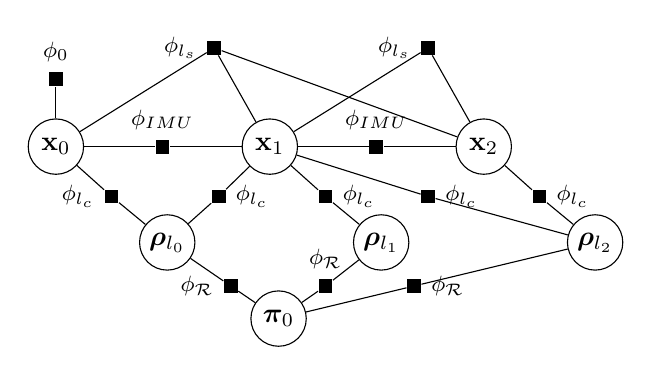
\begin{tikzpicture}
    % X nodes
    \node[latent] (x0) {$\mathbf{x}_0$};
    \node[latent, right= of x0, xshift=\state] (x1) {$\mathbf{x}_1$};
    \node[latent, right= of x1, xshift=\state] (x2) {$\mathbf{x}_2$};

    % L nodes
    \node[latent, below=0.5 of x0, xshift=1.414\state] (l0) {$\bm\rho_{l_0}$};
    \node[latent, below=0.5 of x1, xshift=1.414\state] (l1) {$\bm\rho_{l_1}$};
    \node[latent, below=0.5 of x2, xshift=1.414\state] (l2) {$\bm\rho_{l_2}$};

    % Pi nodes
    \node[latent, below=0.25 of l0, xshift=1.414\state] (pi0) {$\bm\pi_0$};

    % Prior on X0
    \factor[above=of x0, xshift=0\state] {x0prior} {above:$\phi_{0}$} {x0} {}; %

    % Pre-integrated IMU
    % For X0 - X1
    \factor[right=of x0, xshift=0.5\state] {x0-x1} {above:$\phi_{IMU}$} {x0, x1} {}; %
    % For X1 - X2
    \factor[right=of x1, xshift=0.5\state] {x1-x2} {above:$\phi_{IMU}$} {x1, x2} {}; %

    % Landmark observations
    % For L0
    \factor[below=0.18 of x0, xshift=0.707\state] {x0-l0} {left:$\phi_{l_c}$} {x0, l0} {}; %
    \factor[below=0.18 of x1, xshift=-0.650\state] {x1-l0} {right:$\phi_{l_c}$} {x1, l0} {}; %

    % For L1
    \factor[below=0.18 of x1, xshift=0.707\state] {x1-l1} {right:$\phi_{l_c}$} {x1, l1} {}; %

    % For L2
    \factor[below=0.18 of x2, xshift=0.707\state] {x2-l2} {right:$\phi_{l_c}$} {x2, l2} {}; %
    \factor[below=0.18 of x2, xshift=-0.707\state] {x1-l2} {right:$\phi_{l_c}$} {x1, l2} {}; %

    % For structureless
    \factor[above=0.8of x1, xshift=-0.707\state] {x0-x1-x2} {left:$\phi_{l_s}$} {x0, x1,x2} {}; %
    \factor[above=0.8of x2, xshift=-0.707\state] {x1-x2} {left:$\phi_{l_s}$} {x1,x2} {}; %

    % For plane
    % plane-landmarks
    \factor[below=0.1 of l0, xshift=0.807\state] {pi0-l0-l1} {left:$\phi_{\mathcal{R}}$} {l0, pi0} {}; %
    \factor[below=0.1of l1, xshift=-0.707\state] {pi0-l1} {above:$\phi_{\mathcal{R}}$} {l1, pi0} {}; %
    \factor[below=0.1of l2, xshift=-2.3\state] {pi0-l2} {right:$\phi_{\mathcal{R}}$} {l2, pi0} {}; %
  \end{tikzpicture}
  \caption{VIO factor graph combining Structureless ($\phi_{l_s}$), Projection ($\phi_{l_c}$) and Regularity ($\phi_{\mathcal{R}}$) factors (SPR).
The factor $\phi_{\mathcal{R}}$ encodes relative constraints between a landmark $l_i$ and a plane $\pi_0$.}
  \label{fig:factor_graph_s_p_r_1}
\end{figure}

\subsubsection{MAP Estimation}
\label{sssec:map_estimation}
Since we are only interested in the most likely state $\calX_t$ given the measurements $\mathcal{Z}_t$, we calculate the \emph{maximum a posteriori} (MAP) estimator $\calX_t^{\text{MAP}}$.
Maximizing $\calX_t^{\text{MAP}}$ is nevertheless not as convenient as minimizing the negative logarithm of the posterior probability, which, using \cref{eq:factor_form}, simplifies to \cref{eq:simplified_map} for zero-mean Gaussian noise:

\begin{equation}
  \begin{split}
   &\calX_t^{\text{MAP}} = \arg\min_{\calX_t} \normsq{\mathbf{r}_0}{\Sigma_0} + \!\!\!\sum_{l_c\in\Lambda_t}\!\sum_{\pi\in\Pi_t}\delta(l_c, \pi)\normsq{\mathbf{r}_{\mathcal{R}}}{\Sigma_{\mathcal{R}}} \\
                  &+ \!\!\!\!\!\sum_{(i,j)\in\calK_t}\!\!\!\normsq{\mathbf{r}_{\measimu_\subimu}}{\Sigma_{ij}} \!\!\! + \!\!\! \sum_{i\in\calK_t}\!\!\Bigg\{\!\sum_{l_c\in\meascam_i} \normsq{\mathbf{r}_{\mathcal{C}_{i}^{l_c}}}{\Sigma_\mathcal{C}} \!\!\! + \!\!\! \sum_{l_s\in\meascam_i} \normsq{\mathbf{r}_{\mathcal{C}_{i}^{l_s}}}{\Sigma_\mathcal{C}}\!\!\Bigg\} \\
  \end{split}
  \label{eq:simplified_map}
\end{equation}
where $\mathbf{r}$ represents the residual errors, and $\mathbf{\Sigma}$ the covariance matrices.
We refer the reader to \cite[Sec. VI, VII]{Forster17troOnmanifold} for the actual formulation of the preintegrated IMU factors $\phi_{\text{IMU}}$ and structureless factors $\phi_{l_s}$, as well as the underlying residual functions $\mathbf{r}_{\text{IMU}}$, $\mathbf{r}_{C_i^{l_s}}$.
For the projection factors $\phi_{l_c}$, we use a standard monocular and stereo reprojection error formulation as in \cite{Carlone17icra-vioAttention}.

\subsubsection{Regularity Constraints}
\label{sssec:regularity_constraints}

For the regularity factors $\phi_{\mathcal{R}}$, we use a co-planarity constraint between a landmark $\bm\rho_{l_c}\in\mathbb{R}^3$ and a plane $\pi = \{\bm{n}, d\}$, where $\bm{n}$ is the normal of the plane, which lives in the $\Stwo\doteq\{\mathbf{n} = (n_x, n_y, n_z)^T \big| \|\mathbf{n}\| = 1\}$ manifold, and $d\in\mathbb{R}$ the distance to the origin:
$\textstyle\residual_{\mathcal{R}} = \bm{n} \cdot \bm{\rho}_{l_c} - d$.
Representing a plane by its normal and distance to the origin is an over-parametrization that will lead to an information matrix that is singular.
This is not amenable for Gauss-Newton optimization, since it leads to singularities in the normal equations~\cite{Kaess15icra}.
%which requires the inverse of the information matrix.
To avoid the over-parametrization problem, we optimize in the tangent space $T_{\Normal}S^2 \sim \Real^{2}$ % \doteq \big\{\hat\xi \in \Real^3 | \Normal^T \hat\xi = 0\big\}$
of $S^2$ and define a suitable retraction $\calR_{\Normal}(\bm{v}): T_{\Normal}S^2 \in \mathbb{R}^2 \rightarrow \Stwo$
to map changes in the tangent space to changes to the normals in $\Stwo$~\cite{Forster17troOnmanifold}. % to obtain a minimal parametrization for the
In other words, we rewrite the residuals as:
\begin{equation}
  % \residual_\mathcal{R}(\Normal, d) = \Normal^\transpose \cdot \landmark - d \Leftrightarrow
  \residual_\mathcal{R}(\bm{v},d) = \calR_{\Normal}(\bm{v})^\transpose \cdot \landmark - d
  \label{eq:coplanarity_constraint}
\end{equation}
and optimize with respect to the minimal parametrization $\bm{v}$.
 This is similar to the proposal of Kaess~\cite{Kaess15icra}, but we work on the manifold $\Stwo$, while Kaess adopts a quaternion parametrization.
Note that, a single co-planarity constraint, as defined in \cref{eq:coplanarity_constraint}, is not sufficient to constrain a plane variable, and a minimum of three are needed instead.
Nevertheless, degenerate configurations exist, e.g.~three landmarks on a line would not fully constrain a plane.
Therefore, we ensure that a plane candidate has a minimum number of constraints before adding it to the optimization problem.
%\subsubsection{Robust Cost Functions}
%\label{sssec:robust_cost_functions}
\TODO{Do we need to mention robust cost functions at all? I think so, reviews were picky about outliers!}
%Running a feature-based VIO pipeline over planar surfaces, such as walls, has the inconvenience that few features are usually present (i.e. textureless walls), or features are easy to wrongly associate against each other (i.e. a wall with high-frequency texture).
%This can lead to certain estimated landmarks being plainly wrong (outliers), and can consequently corrupt the estimated variables in the optimization problem.
%This is especially problematic in least-squares optimization, which is particularly sensitive to outliers.

%For this reason, we will be using a robust cost function for both the projection and regularity residuals.
%In particular, we found the Huber norm to yield the best results, while we also experimented with the Tukey norm.
%More details on the norm's formulations can be found in \cite{Zhang97ivc}.
%\TODO{Someone may ask why we did not use a robust cost function for structureless factors? And I do not fully understand the underlying mechanism to avoid outliers as it is in our pipeline right now for smart factors...}

%%%%%%%%%%%%%%%%%%%%%%%%%%%%%%%%%%%%%%%%%%%%%%%%%%%%%%%%%%%%%%%%%%%%%%%%%%%%%%%%%%%%

%!TEX root = ../main.tex

\section{Experimental Results}
\label{sec:results}

%The output of our pipeline is two fold: the pose of the camera at each timestep and a mesh-based representation of the scene.
%To quantify the performance of the pose estimate we will be using both absolute and relative error metrics.
%These metrics will give us insights, respectively, on the global and local consistency of the trajectory estimate (\cref{ssec:state_estimation}).
%For the quality of the mesh we will be using a point cloud to point cloud distance as a metric to quantify how well the mesh represents the actual scene (\cref{ssec:mapping_quality}).
%We will also assess the real-time performance of the pipeline in \cref{ssec:timing}.
We benchmark the proposed approach against the state of the art on real datasets, and evaluate
 trajectory and map estimation accuracy, as well as runtime.
We use the \Euroc dataset~\cite{Burri15ijrr}, which contains visual and inertial data recorded from an micro aerial vehicle flying indoors.
The \Euroc dataset includes eleven datasets in total, recorded in two different scenarios.
The \textit{Machine Hall} scenario (\texttt{MH}) is the interior of an industrial facility.
It contains very little (planar) regularities.
The \textit{Vicon Room} (\texttt{V}) is similar to an office room where walls, floor and ceiling are close together, and other planar surfaces are visible
(boxes, stacked mattresses).
Datasets \texttt{V1} and \texttt{V2} differ only by the position of the objects in the scene.
%Moreover, each dataset is labelled by the level of difficulty it represents for Visual-Inertial SLAM algorithms: using the adjectives ``easy", ``medium", and ``difficult".
%The difficulty is increased by simply increasing the speed of the MAV, which results in motion-blur and drastic illumination changes on the images.
%For example, dataset \texttt{MH\_03\_medium} corresponds to a dataset in the Machine Hall where the MAV was flying at moderate speeds.
Each dataset provides the ground truth trajectory of the drone, allowing us to evaluate the accuracy of our estimation.
%compare our estimated trajectory with the real one.
For the \texttt{V} datasets, we are also provided with a ground truth point cloud of the scene, which we use to evaluate the accuracy of our mesh.

\mysubsection{Compared techniques}
To assess the advantages of our proposed approach, we compare three formulations that build one on top of the other.
First, we denote as \textbf{S}, the approach that would neither use regularity factors, nor projection factors, but only use Structureless factors ($\phi_{l_s}$, in \cref{eq:factor_form_c}).
Second, we denote as \textbf{SP}, the approach which would use Structureless factors, combined with Projection factors for those landmarks that have co-planarity constraints ($\phi_{l_c}$, in \cref{eq:factor_form_c}), but without using regularity factors.
Finally, we denote as \textbf{SPR}, our proposed formulation using Structureless, Projection and Regularity factors ($\phi_{\mathcal{R}}$, in \cref{eq:factor_form_a}).
The IMU factors ($\phi_{\text{IMU}}$, in \cref{eq:factor_form_b}) are implicitly used in all three formulations.
We also compare our results with other state-of-the-art implementations in \cref{tab:ape_accuracy_comparison_sopa}.
In particular, we compare the Root Mean Squared Error (RMSE) of our pipeline against OKVIS~\cite{Leutenegger13rss}, MSCKF~\cite{Mourikis07icra},
 ROVIO~\cite{Blosch15iros}, VINS-MONO~\cite{Qin17arxiv}, and SVO-GTSAM~\cite{Forster17troOnmanifold}, using the reported values in~\cite{Delmerico18benchmark}.
We refer the reader to \cite{Delmerico18benchmark} for details on the particular implementations and set of parameters used for each algorithm.
Note that these algorithms use a monocular camera, while we use a stereo camera.
Therefore, while \cite{Delmerico18benchmark} aligns the trajectories using $\mathrm{Sim}(3)$, we use instead $\mathrm{SE}(3)$.
Nevertheless, the scale is observable for all algorithms since they use an IMU.
We only report the values for VINS-MONO when its loop-closure module is disabled.

\subsection{Localization Performance}
\label{ssec:state_estimation}

%  One of the most important outputs of a VIO algorithm is an estimate of the
The state of our optimization problem comprises the poses of the IMU, the velocities, the IMU biases, the planes' parameters, and the landmarks' positions.
In this section we start by benchmarking the quality of the trajectory estimates, which are of paramount importance for control and AR/VR applications.
 The plane and landmark estimates will be assessed in the next \cref{ssec:mapping_quality}, where we evaluate the quality of the mesh.
We will assess the quality of the plane and landmark estimates in Section~\ref{ssec:mapping_quality}.

\mysubsection{Performance Metrics: Absolute Translation Error (ATE)}
\label{ssec:absolute_pose_error}
ATE looks at the translational part of the relative pose between the ground truth pose and the corresponding estimated pose at a given timestamp.
We first align our estimated trajectory with the ground truth trajectory both temporally and spatially (in SE(3)), as explained in \cite[Sec. 4.2.1]{RosinolMT}.
We refrain from using the rotational part since the trajectory alignment ignores the orientation of the pose estimates.
\Cref{tab:ape_all_datasets_pipelines} shows the ATE for our pipeline when using the pipelines S, SP, and our proposed approach SPR on the \Euroc dataset.

First, if we look at the performance of the different algorithmic variants for the datasets \texttt{MH\_03}, \texttt{MH\_04} and \texttt{MH\_05} in \cref{tab:ape_all_datasets_pipelines}, we observe that all methods perform equally.
This is because in these datasets no structural regularities were detected.
Hence, the proposed pipeline SPR gracefully downgrades to a standard structureless VIO pipeline (S).
Second, looking at the results
 for dataset \texttt{V2\_03}, we observe that both the SP and the SPR pipeline achieve the exact same performance.
In this case, structural regularities are detected, resulting in Projection factors being used.
Nevertheless, since the number of regularities detected is not sufficient to spawn a new plane estimate,
no structural regularities are actually enforced in the factor graph.
Finally, \cref{tab:ape_all_datasets_pipelines} shows that the SPR pipeline consistently achieves better results over the rest of datasets where structural regularities are detected and enforced.
In particular, the performance of SPR increases up to 28\% on the median ATE compared to the SP pipeline for datasets with multiple planes (e.g. \texttt{V1} and \texttt{V2}).

%We also divide the MAE by the length of the trajectory in order to be able to compare the performance between different datasets:
%\begin{equation}
  %\label{eq:ape_mae_percent}
  %\mathrm{Drift (\%)} = \frac{\frac{1}{N} \sum_{i=1}^N APE_i}{L},
%\end{equation}
%where $L$ is the length of the trajectory.

%\TODO{I still find this Drift misleading at best, at worst not representative of actual drift...
%We should be integrating the distance from start to point $i$ and dividing each $APE_i$ by this amount?}


\Cref{tab:ape_accuracy_comparison_sopa} shows that our approach, using structural regularities (SPR), achieves the best results when compared with the state-of-the-art,
 on datasets with structural regularities, such as in datasets \texttt{V1\_01\_easy} and \texttt{V1\_02\_medium},
  where multiple planes are present (walls, floor).
    We observe a $19\%$ improvement compared to the next best performing algorithm (SVO-GTSAM) in dataset \texttt{V1\_01\_easy},
     and a $26\%$ improvement in dataset \texttt{V1\_02\_medium} compared to ROVIO and VINS-MONO, which achieve the next best results.
    We also see that the performance of our pipeline is on-par with other state-of-the-art approaches when no structural regularities are present, such as in datasets \texttt{MH\_04\_difficult} and \texttt{MH\_05\_difficult}.

%\TODO{Important detail that I avoided altogether is that we are using the stereo camera also, while the above pipelines are all monocular. I just didn't mention stereo because then I have to add the stereo factors which make the whole story longer (Projection factors would now be mono/stereo etc).}
%Finally, we found to be instructive to color-code the estimated trajectory with the actual ATE errors at each pose estimate; which provides insights on how quickly the state estimation degrades.
%We provide these plots in the appendix of the thesis \TODO{cite Master's Thesis}.

% APE boxplots.
%\begin{figure*}[htbp]
  %\centering     %%% not \center
  %\includegraphics[trim={0 0 0 0cm},clip,width=0.7\textwidth]{datasets_ape_boxplots.eps}
  %\caption{Comparison of the Absolute Pose Error (APE) on the \Euroc{} datasets while using Structureless factors (S), Structureless and Projection factors (SP), and our proposed approach using Structureless, Projection and Regularity factors (SPR).}
  %\label{fig:ape_all_datasets_pipelines}
%\end{figure*}

% APE table results.
\begin{table}[tb]
  \centering
  \caption{ATE for pipelines S, SP, and SPR. Our proposed approach SPR achieves the best results for all datasets where structural regularities are detected and enforced.}
  \label{tab:ape_all_datasets_pipelines}
  \begin{tabularx}{\columnwidth}{l *6{Y}}
    \toprule
    & \multicolumn{6}{c}{ATE [cm]} \\
    \cmidrule{2-7}
    & \multicolumn{2}{c}{S} & \multicolumn{2}{c}{SP} & \multicolumn{2}{c}{SPR (\textbf{Proposed})} \\
    \cmidrule(r){2-3} \cmidrule(){4-5} \cmidrule(l){6-7}
    EuRoC Sequence & Median & RMSE & Median & RMSE & Median & RMSE \\
    \midrule
                 %MH\_01\_easy & 13.7 & 15.0 & 12.4 & 15.0 & \textbf{{10.7}} & \textbf{{14.5}} \\
             %MH\_02\_easy & 12.9 & 13.1 & 17.6 & 16.7 & \textbf{{12.6}} & \textbf{{13.0}} \\
           %MH\_03\_medium & 21.0 & 21.2 & 21.0 & 21.2 & 21.0 & 21.2 \\
        %MH\_04\_difficult & 17.3 & 21.7 & 17.3 & 21.7 & 17.3 & 21.7 \\
        %MH\_05\_difficult & 21.6 & 22.6 & 21.6 & 22.6 & 21.6 & 22.6 \\
             %V1\_01\_easy & 5.6 & 6.4 & 6.2 & 7.7 & \textbf{{5.3}} & \textbf{{5.7}} \\
           %V1\_02\_medium & 7.7 & 8.9 & 8.7 & 9.4 & \textbf{{6.3}} & \textbf{{7.4}} \\
        %V1\_03\_difficult & 17.7 & 23.1 & 13.6 & 17.6 & \textbf{{13.5}} & \textbf{{16.7}} \\
             %V2\_01\_easy & 8.0 & 8.9 & 6.6 & 8.2 & \textbf{{6.3}} & \textbf{{8.1}} \\
           %V2\_02\_medium & 8.8 & 12.7 & 9.1 & 13.5 & \textbf{{7.1}} & \textbf{{10.3}} \\
        %V2\_03\_difficult & 37.9 & 41.5 & 26.0 & 27.2 & 26.0 & 27.2 \\
                 %MH\_01\_easy & 13.7 & 15.0 & 12.4 & 15.0 & \textbf{{10.7}} & \textbf{{14.5}} \\

             MH\_02\_easy & 12.9 & 13.1 & 17.6 & 16.7 & \textbf{{12.6}} & \textbf{{13.0}} \\
             MH\_03\_medium & \textbf{21.0} & \textbf{21.2} & \textbf{21.0} & \textbf{21.2} &\textbf{21.0} & \textbf{21.2} \\
             MH\_04\_difficult & \textbf{17.3} & \textbf{21.7} & \textbf{17.3} & \textbf{21.7} & \textbf{17.3} &  \textbf{21.7} \\
             MH\_05\_difficult & \textbf{21.6} & \textbf{22.6} & \textbf{21.6} & \textbf{22.6} & \textbf{21.6} &  \textbf{22.6} \\
             V1\_01\_easy & 5.6 & 6.4 & 6.2 & 7.7 & \textbf{{5.3}} & \textbf{{5.7}} \\
           V1\_02\_medium & 7.7 & 8.9 & 8.7 & 9.4 & \textbf{{6.3}} & \textbf{{7.4}} \\
        V1\_03\_difficult & 17.7 & 23.1 & 13.6 & 17.6 & \textbf{{13.5}} & \textbf{{16.7}} \\
             V2\_01\_easy & 8.0 & 8.9 & 6.6 & 8.2 & \textbf{{6.3}} & \textbf{{8.1}} \\
           V2\_02\_medium & 8.8 & 12.7 & 9.1 & 13.5 & \textbf{{7.1}} & \textbf{{10.3}} \\
           V2\_03\_difficult & 37.9 & 41.5 & \textbf{26.0} & \textbf{27.2} & \textbf{26.0} & \textbf{27.2} \\
    \bottomrule
  \end{tabularx}%
\end{table}


% V1_01_easy
%\begin{figure}[htbp]
  %\centering

  %\begin{subfigure}[c]{0.7\columnwidth}
    %\resizebox{\columnwidth}{!}{\inputpgf{./results/V1_01_easy/SP/}{plots_APE_translation_trajectory_error.pgf}}
    %\subcaption{APE translation for S+P}
  %\end{subfigure}

  %\begin{subfigure}[c]{0.7\columnwidth}
    %\resizebox{\columnwidth}{!}{\inputpgf{./results/V1_01_easy/SPR/}{plots_APE_translation_trajectory_error.pgf}}
    %\subcaption{APE translation for S+PR}
  %\end{subfigure}

  %\caption{Dataset \texttt{V1\_01\_easy}: APE translation error plotted on the trajectory estimated by VIO using Strutureless and Projection factors (S + P), against our proposed approach using also Regularity factoris (S + P + R).}
  %\label{fig:ape_trans_traj_V1_01_easy}
%\end{figure}

%\begin{figure}[htbp]
  %\centering

  %\begin{subfigure}[c]{0.7\columnwidth}
    %\resizebox{\columnwidth}{!}{\inputpgf{./results/V1_01_easy/SP/}{plots_APE_translation.pgf}}
    %\subcaption{S+P}
  %\end{subfigure}

  %\begin{subfigure}[c]{0.7\columnwidth}
    %\resizebox{\columnwidth}{!}{\inputpgf{./results/V1_01_easy/SPR/}{plots_APE_translation.pgf}}
    %\subcaption{S+P+R}
  %\end{subfigure}

  %\caption{Dataset \texttt{V1\_01\_easy}: APE translation error of VIO using Strutureless and Projection factors (S + P), against our proposed approach using Structureless, Projection and Regularity factors (S +P + R).}
  %\label{fig:ape_trans_V1_01_easy}
%\end{figure}

% APE against state-of-the-art pipelines.

\begin{table}[tb]
  \centering
  \caption{ATE's RMSE of the state-of-the-art techniques (reported values from \cite{Delmerico18benchmark}) compared to our proposed SPR pipeline, on the \Euroc dataset. A cross ($\times$) states that the pipeline failed.
  In \textbf{bold} the best result, in \textcolor{blue}{blue} the second best.}
  \label{tab:ape_accuracy_comparison_sopa}
  \begin{tabularx}{\columnwidth}{l *6{Y}}
    \toprule
    & \multicolumn{6}{c}{RMSE ATE [cm]} \\
    \cmidrule(l){2-7}
    Sequence  & OKVIS & MSCKF & ROVIO & VINS-MONO & SVO-GTSAM & \textbf{SPR} \\
    \midrule
    MH\_01\_e & 16 & 42 & 21 & 27 & \textbf{5} & \textbf{\textcolor{blue}{14}} \\
    MH\_02\_e & 22 & 45 & 25 & \textbf{\textcolor{blue}{12}} & \textbf{3} & 13 \\
    MH\_03\_m & 24 & 23 & 25 & \textbf{\textcolor{blue}{13}} & \textbf{12} & 21 \\
    MH\_04\_d & 34 & 37 & 49 & 23 & \textbf{13} & \textbf{\textcolor{blue}{22}} \\
    MH\_05\_d & 47 & 48 & 52 & 35 & \textbf{16} & \textbf{\textcolor{blue}{23}} \\
    V1\_01\_e & 9 & 34 & 10 & \textbf{\textcolor{blue}{7}} & \textbf{\textcolor{blue}{7}} & \textbf{6} \\
    V1\_02\_m & 20 & 20 & \textbf{\textcolor{blue}{10}} & \textbf{\textcolor{blue}{10}} & 11 & \textbf{7} \\
    V1\_03\_d & 24 & 67 & \textbf{\textcolor{blue}{14}} & \textbf{13} & $\times$ & 17 \\
    V2\_01\_e & 13 & 10 & 12 & \textbf{\textcolor{blue}{8}} & \textbf{7} & \textbf{\textcolor{blue}{8}} \\
    V2\_02\_m & 16 & 16 & 14 & \textbf{8} & $\times$ & \textbf{\textcolor{blue}{10}} \\
    V2\_03\_d & 29 & 113 & \textbf{14} & \textbf{\textcolor{blue}{21}} & $\times$ & 27 \\
    \bottomrule
  \end{tabularx}%
\end{table}


    %MH\_01\_e & 16 & 42 & 21 & 27 & \textbf{5} & 14.5 \\
    %MH\_02\_e & 22 & 45 & 25 & 12 & \textbf{3} & 13.0 \\
    %MH\_03\_m & 24 & 23 & 25 & 13 & \textbf{12} & 21.2 \\
    %MH\_04\_d & 34 & 37 & 49 & 23 & \textbf{13} & 21.7 \\
    %MH\_05\_d & 47 & 48 & 52 & 35 & \textbf{16} & 22.6 \\
    %V1\_01\_e & 9 & 34 & 10 & 7 & 7 & \textbf{5.7} \\
    %V1\_02\_m & 20 & 20 & 10 & 10 & 11 & \textbf{7.4} \\
    %V1\_03\_d & 24 & 67 & 14 & \textbf{13} & $\times$ & 16.7 \\
    %V2\_01\_e & 13 & 10 & 12 & 8 & \textbf{7} & 8.1 \\
    %V2\_02\_m & 16 & 16 & 14 & \textbf{8} & $\times$ & 10.3 \\
    %V2\_03\_d & 29 & 113 & \textbf{14} & 21 & $\times$ & 27.2 \\

%\TODO{Say that in datasets where there are no structural regularities we are actually comparing our non-regular pipeline implementation against the others... but ours has not been optimized...}

\mysubsection{Performance Metrics: Relative Pose Error (RPE)}
\label{ssec:relative_pose_error}
While the ATE provides information on the global consistency of the trajectory estimate, it does not provide insights on the moment in time when the erroneous estimates happen.
Instead, the Relative Pose Error (RPE) is a metric for investigating the local consistency of a SLAM trajectory.
RPE aligns the estimated and ground truth pose for a given frame $i$, and then computes the error of the estimated pose for a frame $j>i$ at a fixed distance farther along the trajectory.
We calculate the RPE from frame $i$ to $j$ in translation and rotation (absolute angular error) \cite[Sec. 4.2.3]{RosinolMT}.
As \cite{Geiger12cvpr}, we evaluate the RPE over all possible trajectories of a given length, and for different lengths.
Nevertheless, instead of calculating the mean of all RPE for a given trajectory length, we report the maximum, the minimum, the first and third quartile, as well as the median.

\mysubsection{RPE results}
In \Cref{fig:boxplot_rpe}, we show the results for dataset \texttt{V2\_02}, where we observe that using our proposed pipeline SPR, with respect to the SP pipeline, leads to: (i) an accuracy improvement of up to 50\% in translation and 30\% in rotation (based on the maximum improvement on the median of the errors), and, (ii) an average improvement over all trajectory lenghts of 20\% in translation and 15\% in rotation (for the median errors).

%\begin{figure}[htbp]
  %\centering     %%% not \center

  %\begin{subfigure}[c]{0.7\columnwidth}
    %\includegraphics[trim={0 0 0 0cm},clip,width=\columnwidth]{./results/MH_03_medium/traj_relative_errors_boxplots.eps}
    %\subcaption{\texttt{MH\_03\_medium}}
    %\label{fig:boxplot_rpe_mh_03_v2_03_subfig_a}
  %\end{subfigure}
  %\begin{subfigure}[c]{0.7\columnwidth}
    %\includegraphics[trim={0 0 0 0cm},clip,width=\columnwidth]{./results/v2_03_difficult/traj_relative_errors_boxplots.eps}
    %\subcaption{\texttt{V2\_03\_difficult}}
    %\label{fig:boxplot_rpe_mh_03_v2_03_subfig_b}
  %\end{subfigure}

  %\caption{Detailed comparison of the state estimation accuracy while using Structureless factors (S), Structureless and Projection factors (SP), and our proposed approach using Structureless, Projection and Regularity factors (SPR) on \Euroc{}'s V1\_02\_medium and V2\_02\_medium datasets.}

  %\label{fig:boxplot_rpe_mh_03_v2_03}
%\end{figure}

\begin{figure}[htbp]
  \centering     %%% not \center

    %\includegraphics[trim={0 13.5cm 0 0cm},clip,width=0.5\columnwidth]{./results/V1_02_medium/traj_relative_errors_boxplots.eps}
    %\includegraphics[trim={0.1cm 0 0.05cm 1.25cm},clip,width=0.52\columnwidth]{./results/V1_02_medium/traj_relative_errors_boxplots.eps}
    %\hspace{-1em}
    %\includegraphics[trim={1.0cm 0 0.2cm 1.25cm},clip,width=0.4605\columnwidth]{./results/V2_02_medium/traj_relative_errors_boxplots.eps}
    %\includegraphics[trim={0cm 0 0cm 0cm},clip,width=\columnwidth]{./results/V1_02_medium/traj_relative_errors_boxplots.eps}
    \includegraphics[trim={0.1cm 0 0cm 0.2cm},clip,width=0.8\columnwidth]{./results/V2_02_medium/traj_relative_errors_boxplots.eps}

  \caption{Detailed comparison of the state estimation accuracy while using pipeline S, SP, and our proposed approach SPR on different \Euroc{} datasets.}

  \label{fig:boxplot_rpe}
\end{figure}

\subsection{Mapping quality}
\label{ssec:mapping_quality}
We use the ground truth point cloud for \texttt{V1} dataset to assess the quality of the mesh by calculating its \textit{accuracy} as defined in \cite{Schoeps2017cvpr}.

\mysubsection{Performance Metric: Map Accuracy}
  \label{ssec:map_accuracy}
%   by calculating its \textit{accuracy} %(\cref{ssec:map_accuracy})
% as defined in \cite{Schoeps2017cvpr}.
Comparing a mesh with a dense point cloud can be achieved by generating a point cloud from the mesh itself, and then comparing both point clouds.
In our case, we compute a point cloud by sampling the mesh with a uniform density of $10^3$ points per square meter.
We also register the resulting point cloud to the ground truth point cloud using an iterative closest point algorithm.
%
%\TODO{Here we are not saying how we merge sparse meshes together for evaluation (we are not just appending time-horizon meshes together...)}
  With the newly registered point cloud, we can compute a cloud to cloud distance to assess the accuracy of the mesh relative to the ground truth point cloud.
  More specifically, for each point $r$ of the estimated cloud from the mesh $\mathcal{R}$, we search the nearest point in the ground truth cloud $\mathcal{G}$, and compute their Euclidean distance $d_{r \to \mathcal{G}}$:

  \begin{equation}
    \label{eq:c2c_distance}
    d_{r \to \mathcal{G}} = \min_{g \in \mathcal{G}}\left\|{r-g}\right\|_{2} \quad\text{for}\quad r \in \mathcal{R}.
  \end{equation}

  \Cref{tab:mesh_accuracy_stats_comparison} shows that both the mean and the standard deviation of the distance from the mesh to the ground truth point cloud (\cref{eq:c2c_distance}) decreases when enforcing structural regularities, as done in the SPR pipeline.
  On average, each point sampled on the mesh generated by the SPR pipeline is $0.5$ cm closer to the ground truth point cloud than the points sampled on the mesh generated by the SP pipeline.
  Therefore, enforcing structural regularities makes the estimated mesh closer to the real scene.

  We also report the accuracy $\mathcal{A}(\tau)$, defined as the fraction of estimated points which are within a distance threshold $\tau$ of the ground truth point cloud \cite{Schoeps2017cvpr, Knapitsch2017}:
  \begin{equation}
    \label{eq:mesh_accuracy}
    \mathcal{A}(\tau) = \frac{1}{|\mathcal{R}|}\sum_{r \in \mathcal{R}}\bigg[d_{r \to \mathcal{G}} < \tau\bigg]_I \times 100,
  \end{equation}
  where $[P]_I$ is the Iverson bracket, defined as:
  \begin{equation*}
    [P]_I={\begin{cases}
        1&{\text{if }}P{\text{ is true;}}\\
        0&{\text{otherwise,}}
    \end{cases}}
  \end{equation*}

  \Cref{fig:histogram_accuracy_mesh} shows the actual error distributions for $d_{r \to \mathcal{G}}$, and the mesh accuracy $\mathcal{A}(\tau)$ for different distance thresholds $\tau$, for both the SP and the SPR pipelines respectively.
  In terms of accuracy values $\mathcal{A}(\tau)$, we can see in \cref{fig:histogram_accuracy_mesh} that the SPR pipeline consistently achieves more accurate mesh estimates (between 3\%-7\% better) for distance thresholds $\tau < 10cm$.

  As a reminder, the SP pipeline still uses the mesh to detect regularities, but, contrary to the SPR pipeline, it does not enforce the structural regularities on the landmarks.

  In \cref{fig:accuracy_mesh}, we color-encode each point on the estimated point cloud with the error distances $d_{r \to \mathcal{G}}$.
  We can observe that, when we do not enforce structural regularities, significant errors are actually present on the planar surfaces, especially on the walls (\cref{fig:accuracy_mesh} top).
  Instead, when regularities are enforced, the errors on the walls and the floor are reduced (\cref{fig:accuracy_mesh} bottom).
\TODO{Remove everything except this and the results in table 3}  A closer view on the wall itself, bottom figures (c) and (d) of \cref{fig:intro}, shows that it is visually clear that adding co-planarity constraints results in smoother walls.

% Cloud comparison table
\begin{table}[]
  \caption{Statistics for the cloud to cloud absolute distance from the mesh to the ground truth point cloud $d_{r \to \mathcal{G}}$ (\cref{eq:c2c_distance}) for dataset \texttt{V1\_01\_easy}.}
  \label{tab:mesh_accuracy_stats_comparison}
  \centering
  \begin{tabularx}{\columnwidth}{l *2{Y}}%
    \toprule
    & \multicolumn{2}{c}{VIO Type} \\
    \cmidrule(lr){2-3}
    $d_{r \to \mathcal{G}}$ Statistics & SP & SPR (\textbf{Proposed}) \\
    \cmidrule(lr){2-2} \cmidrule(lr){3-3}
    Mean $\bar{d}_{\mathcal{R}}$ [cm] & 4.9 & \textbf{4.4} \\
    Standard Deviation $\sigma_{\mathcal{R}}$ [cm] & 5.0 & \textbf{4.6} \\
    \bottomrule
  \end{tabularx}
\end{table}

% ground truth point cloud.
%\begin{figure}[tb]
%  \centering     %%% not \center
%  \includegraphics[trim={0 0 0 0cm},clip,height=0.5\columnwidth, width=\columnwidth]{./results/gt_point_cloud/V1_01_easy/frames_animation/frame_000000.png}
%  \caption{ground truth point cloud. Color-encoded for better visualization.}
%  \label{fig:ground_truth_point_cloud}
%\end{figure}

% Mesh accuracy histograms
\begin{figure}[tb]
  \centering     %%% not \center
  %\adjustbox{width=\columnwidth,trim=0.0cm 0pt 0.2ex 0pt,clip}{\resizebox{0.49\textwidth}{!}{\inputpgf{./results/S_P_Mesh/Histogram/}{Histogram_for_paper_accuracy_S_P.pgf}}}
  \adjustbox{width=\columnwidth,trim=0.1cm 0 0.1cm 0,clip}{\resizebox{\columnwidth}{!}{\inputpgf{./results/S_P_R_Mesh/Histogram/}{Histogram_for_paper_accuracy_S_P_R.pgf}}}

  %\caption{(Top) Histogram of points sampled on the mesh depending on their distance to the ground truth point cloud ($d_{r \to \mathcal{G}}$) for dataset \texttt{V1\_01\_easy} and pipelines SP (left) and SPR (right).
  %Detailed is the mesh accuracy $\mathcal{A}(\tau)$, as defined in \cref{eq:mesh_accuracy}, for different distance thresholds $\tau$. (Bottom) Color-encoded point cloud sampled from the estimated 3D mesh. The colormap is the same for all figures.}
  \caption{Histogram of points sampled on the mesh depending on their distance to the ground truth point cloud ($d_{r \to \mathcal{G}}$) for dataset \texttt{V1\_01\_easy} and pipelines SP (left) and SPR (right).
  Detailed is the mesh accuracy $\mathcal{A}(\tau)$, as defined in \cref{eq:mesh_accuracy}, for different distance thresholds $\tau$.}
  \label{fig:histogram_accuracy_mesh}
\end{figure}

\subsection{Timing}
\label{ssec:timing}

The pipelines S, SP, and SPR differ in that they try to solve an increasingly complicated problem.
While the S pipeline does not include neither the 3D landmarks nor the planes as variables in the optimization problem, the SP pipeline includes 3D landmarks, and the pipeline using regularities (SPR) further includes planes as variables.
Moreover, the SP has significantly less constraints between the variables than the SPR pipeline.
Hence, we can expect that the optimization times for the different pipelines will be each bounded by the other as $t_{S}^{opt} < t_{SP}^{opt} < t_{SPR}^{opt}$, where $t_{X}^{opt}$ is the time taken to solve the optimization problem of pipeline X.

\Cref{fig:optimization_time} shows the time taken to solve the optimization problem for each type of pipeline.
Experimentally, we observe that the optimization time follows roughly the expected distribution $t_{S}^{opt} < t_{SP}^{opt} < t_{SPR}^{opt}$.
We also observe that if the number of plane variables is large ($\sim 10^1$), and consequently the number of constraints between landmarks and planes also gets large ($\sim 10^2$), the optimization problem cannot be solved in real-time.
For example, for the keyframe index 250 in \Cref{fig:optimization_time}, we can see that a spike is present caused by the detection of multiple planes and landmarks with regularities.

\begin{figure}[tb]
  \centering     %%% not \center
    \resizebox{\columnwidth}{!}{\inputpgf{./img/}{all_timing_for_paper.pgf}}
  \caption{Comparison of the time to solve the optimization problem for pipeline S, SP, and SPR for dataset \texttt{V1\_01\_easy}.}
  \label{fig:optimization_time}
\end{figure}




%!TEX root = ../main.tex

\section{Conclusion}
\label{sec:conclusions}

%\addtolength{\textheight}{-11cm}   % This command serves to balance the column lengths
                                  % on the last page of the document manually. It shortens
                                  % the textheight of the last page by a suitable amount.
                                  % This command does not take effect until the next page
                                  % so it should come on the page before the last. Make
                                  % sure that you do not shorten the textheight too much.


%\section*{Acknowledgments}

\bibliographystyle{IEEEtran} % use IEEEtran.bst style
\bibliography{bibliography}

%\addtolength{\textheight}{0cm}   % This command serves to balance the column lengths
%\newpage
%\input{./chapters/appendix_content.tex}

\end{document}
